\documentclass[aspectratio=169]{beamer}

% --- STILE PULITO E MINIMALE ---
\usetheme{Boadilla}
\usefonttheme{professionalfonts}
\setbeamertemplate{navigation symbols}{} % Rimuove i fastidiosi bottoncini in basso

% --- COLORI POLITECNICO DI MILANO ---
\definecolor{PoliBlue}{RGB}{20, 43, 104}
\definecolor{PoliRed}{RGB}{237, 28, 36}

\setbeamercolor{structure}{fg=PoliBlue}
\setbeamercolor{title}{fg=PoliBlue}
\setbeamercolor{frametitle}{fg=PoliBlue}
\setbeamercolor{item}{fg=PoliBlue}
\setbeamertemplate{items}[triangle]
\setbeamercolor{block title}{bg=PoliBlue, fg=white}
\setbeamercolor{block body}{bg=PoliBlue!10, fg=black}

\usepackage{amsmath, amssymb, graphicx, booktabs, tikz}
\usepackage{colortbl}
\usepackage{array}

% --- CUSTOM COMMANDS FOR BACKUP TABLES ---
\newcommand\T{\rule{0pt}{2.6ex}}
\newcommand\B{\rule[-1.2ex]{0pt}{0pt}}
\definecolor{bluePoli}{RGB}{20, 43, 104}
\newcommand{\maxval}[1]{\cellcolor{orange!25}\textbf{#1}}
\newcommand{\minval}[1]{\cellcolor{blue!15}\textbf{#1}}
\newcolumntype{H}{@{}>{\setbox0=\hbox\bgroup}c<{\egroup}@{}}


% --- DATI INTESTAZIONE ---
\title[Branch Prediction]{Design and Optimization of a High-Performance and Energy-Efficient Branch Predictor in HARCOM}
\subtitle{Advanced Computer Architectures project}
\author[Di Lauro, Ghiotto]{Roberto Di Lauro, Alessandro Ghiotto}
\institute[PoliMi]{Politecnico di Milano - MSc HPC Engineering}
\date{July 2026}

\begin{document}

\begin{frame}
    \titlepage
\end{frame}

\begin{frame}{Outline}
    \tableofcontents
\end{frame}

\section{Introduction}
\begin{frame}{Introduction}
    \begin{block}{Background}
        \begin{itemize}
            \item \textbf{Speculative Execution:} critical for modern superscalar performance.
            \item \textbf{Misprediction Cost:} pipeline flushes cause severe IPC loss and energy waste.
        \end{itemize}
    \end{block}
    \begin{block}{Goals}
        \begin{itemize}
            \item \textbf{Exploration:} benchmark classical global and local history predictors under strict \textbf{8~KB} and \textbf{16~KB} HW budgets.
            \item \textbf{TAGE Proposal:} design and evaluate an optimized low-power version of TAGE (\textbf{TAGE~sat}).
            \item \textbf{Optimization Target:} maximize VFS Speedup (balancing accuracy, latency, and energy over 12 CBP-NG benchmarks).
        \end{itemize}
    \end{block}
\end{frame}

\section{Block-Level Prediction}
\begin{frame}{Block-Level Prediction}
    \begin{columns}[T]
        \column{0.45\textwidth}
        \begin{block}{SRAM Access Amortization}
            \begin{itemize}
                \item \textbf{Scalar Bottleneck:} a SRAM lookup per instruction limits the IPC to less than 1.0.
                \item \textbf{Block Prediction (L):} predicts up to $LI = 16$ instructions in a single wide SRAM row access.
                \item \textbf{Register Reuse:} store active row bits to skip subsequent lookups.
                \item \textbf{Benefits:} increase IPC and decrease EPI.
            \end{itemize}
        \end{block}
        \column{0.5\textwidth}
        \vspace*{-0.15cm}
        \IfFileExists{images/interface-flowchart.pdf}{%
            \begin{center}
                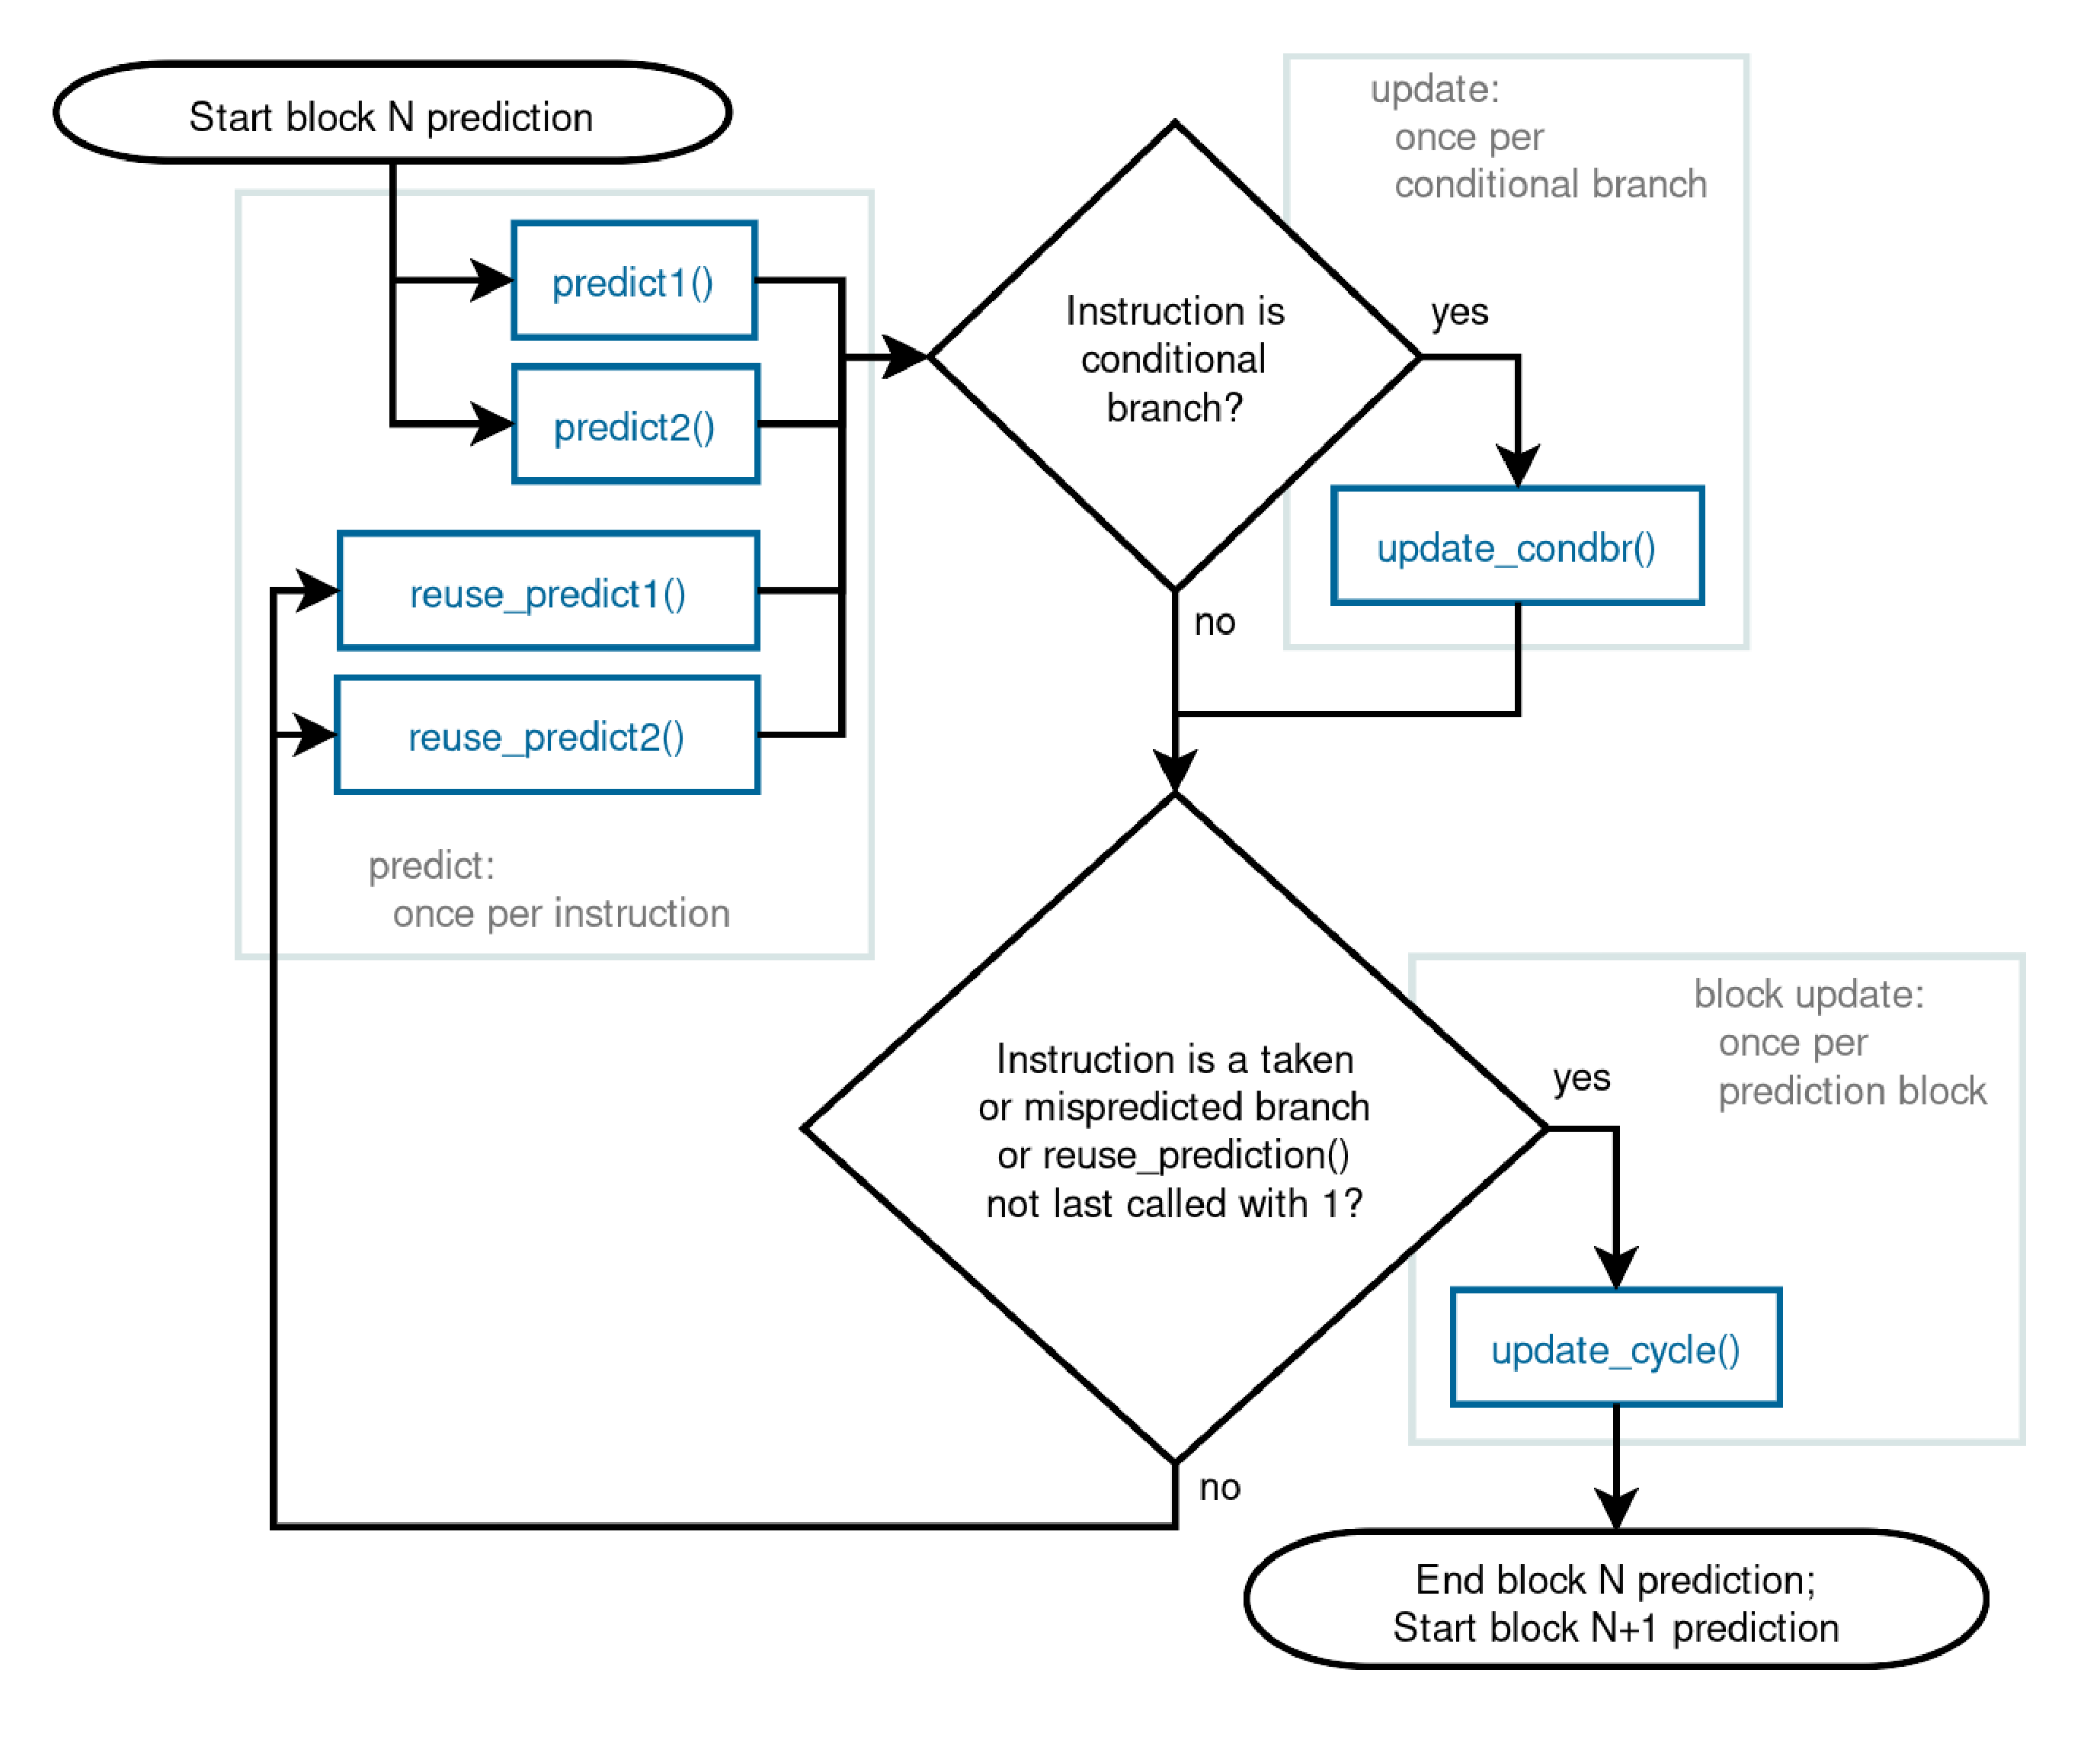
\includegraphics[width=1.08\textwidth, height=7.5cm, keepaspectratio]{images/interface-flowchart.pdf}
            \end{center}
        }{%
            \small\textcolor{gray}{\textit{[predictor interface]}}
        }
        % \begin{block}{Key Benefits}
        %     \begin{itemize}
        %         \item \textbf{IPC Boost:} 3.00--4.85 (vs. 0.49--0.98 for scalar) \hyperlink{main_results}{\beamerbutton{Results}}.
        %         \item \textbf{Energy reduction:} block prediction decreases EPI:
        %         \begin{itemize}
        %             \item Scalar \texttt{gshare}: 263.2 fJ
        %             \item Block \texttt{gshareL}: 145.5 fJ ($\approx 45\%$ savings) \hyperlink{block_16kb}{\beamerbutton{16KB Table}}
        %         \end{itemize}
        %         \item \textbf{VFS Speedup:} Yields a \textbf{3.0x to 5.64x} overall performance increase \hyperlink{speedup_table}{\beamerbutton{Speedup Table}}.
        %     \end{itemize}
        % \end{block}
    \end{columns}
\end{frame}

\section{TAGE}
\begin{frame}{TAGE}
    \small
    \begin{columns}[T]
        \column{0.52\textwidth}
        \begin{block}{Accuracy \& Energy Challenges}
            \begin{itemize}
                % \item \textbf{Geometric History:} captures long-term correlations.
                \item \textbf{Base predictor ($T_0$):} bimodal.
                \item \textbf{3 Tagged Tables ($T_1, T_2, T_3$):} history of 4, 16, 64 bits.
                \item \textbf{Replacement:} useful bit ($u$).
                \item \textbf{Accuracy:} peak at \hyperlink{block_16kb}{\textbf{4.19 MPKI}} (\texttt{tage\_uL}). 
                % \item \textbf{Parallel Lookup:} concurrent reads to $T_1, T_2, T_3$ in Stage 2.
                \item \textbf{High EPI:} \texttt{tageL} at \hyperlink{block_16kb}{\textbf{1145 fJ}} ($\approx 8\times$ vs. \texttt{gshareL}) .
            \end{itemize}
        \end{block}

        \column{0.44\textwidth}
        \vspace*{0.25cm}
        \IfFileExists{images/tage_architecture.png}{%
            \begin{center}
                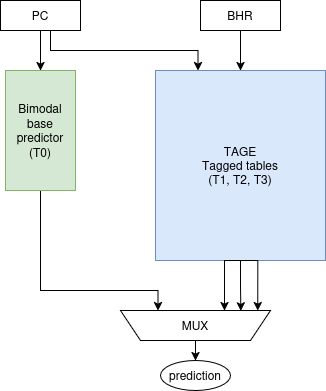
\includegraphics[width=1.04\textwidth, height=6.4cm, keepaspectratio]{images/tage_architecture.png}
            \end{center}
        }{%
            \small\textcolor{gray}{\textit{[TAGE Diagram]}}
        }
    \end{columns}
\end{frame}

\section{Proposed Methodologies}
\subsection{TAGE bimode}
\begin{frame}{Proposed Methodologies: TAGE bimode}
    \small
    \begin{columns}[T]
        \column{0.52\textwidth}
        \begin{block}{Idea}
            \begin{itemize}
                \item \textbf{Choice Table:} splits predictions into separate taken/not-taken tables.
                \item \textbf{Design Role:} integrated as the base table ($T_0$) for the TAGE predictor framework.
            \end{itemize}
        \end{block}
        \vspace{0.05cm}
        \begin{block}{Resource Constraints \& Aliasing}
            \begin{itemize}
                \item \textbf{Storage Overhead:} base table consumes \textbf{64\%} of the total storage budget.
                \item \textbf{Aliasing Penalty:} forces short tags (8-bit) $\rightarrow$ severe aliasing (\textbf{9.74 MPKI}) and high power (\hyperlink{block_16kb}{\textbf{1587 fJ EPI}}).
            \end{itemize}
        \end{block}

        \column{0.44\textwidth}
        \vspace*{-0.15cm}
        \IfFileExists{images/bimode_architecture.png}{%
            \begin{center}
                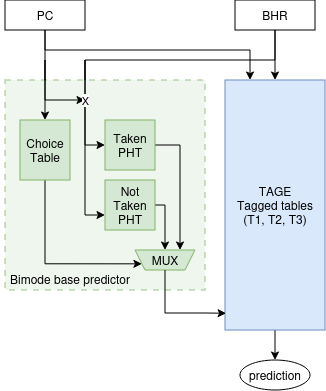
\includegraphics[width=\textwidth, height=6.4cm, keepaspectratio]{images/bimode_architecture.png}
            \end{center}
        }{%
            \small\textcolor{gray}{\textit{[Bi-Mode Diagram]}}
        }
    \end{columns}
\end{frame}

\subsection{TAGE bias}
\begin{frame}{Proposed Methodologies: TAGE bias}
    \small
    \begin{columns}[T]
        \column{0.52\textwidth}
        \begin{block}{Idea}
            \begin{itemize}
                \item \textbf{Bias Filter Table:} employs a dedicated table to identify strongly biased branches.
                \item \textbf{Power Savings:} bypass expensive TAGE SRAM lookups.
            \end{itemize}
        \end{block}
        \vspace{0.05cm}
        \begin{block}{Latency Penalty}
            \begin{itemize}
                \item \textbf{Serialization:} sequential checking of the bias table in Stage 1 extends the critical path.
                \item \textbf{Throughput Drop:} halves the operating frequency $\rightarrow$ IPC drops to \hyperlink{block_16kb}{\textbf{2.83}}.
            \end{itemize}
        \end{block}

        \column{0.44\textwidth}
        \vspace*{-0.15cm}
        \IfFileExists{images/bias_architecture.png}{%
            \begin{center}
                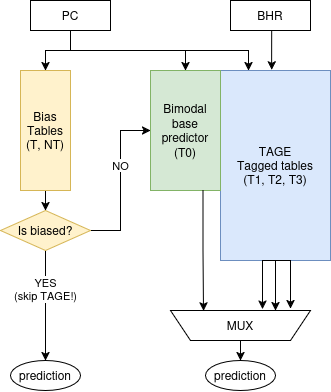
\includegraphics[width=1.06\textwidth, height=6.4cm, keepaspectratio]{images/bias_architecture.png}
            \end{center}
        }{%
            \small\textcolor{gray}{\textit{[Bias Diagram]}}
        }
    \end{columns}
\end{frame}

\subsection{TAGE sat}
\begin{frame}{Our Final Proposal: TAGE sat}
    \small
    \begin{columns}[T]
        \column{0.52\textwidth}
        \begin{block}{Idea}
            \begin{itemize}
                \item \textbf{Bypass Condition:} check if the bimodal base counters is saturated (strongly biased).
                \item \textbf{Dynamic Bypass:} skip tagged SRAM lookups ($t_1, t_2, t_3$).
            \end{itemize}
        \end{block}
        \vspace{0.05cm}
        \begin{block}{Benefits}
            \begin{itemize}
                \item \textbf{Throughput:} bypasses Stage 2 SRAM latency $\rightarrow$ \hyperlink{block_16kb}{\textbf{4.85 IPC}}.
                \item \textbf{Power:} disables tagged table SRAM reads $\rightarrow$ cuts EPI by \hyperlink{block_16kb}{\textbf{14.6\% -- 21.3\%}}.
            \end{itemize}
        \end{block}

        \column{0.44\textwidth}
        \vspace*{-0.25cm}
        \IfFileExists{images/sat_architecture.png}{%
            \begin{center}
                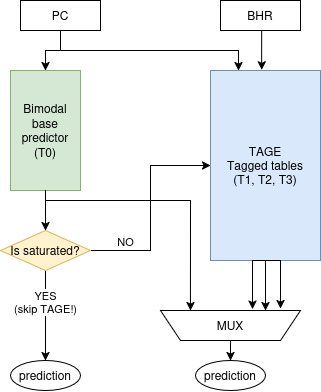
\includegraphics[width=1.04\textwidth, height=6.4cm, keepaspectratio]{images/sat_architecture.png}
            \end{center}
        }{%
            \small\textcolor{gray}{\textit{[TAGE sat Diagram]}}
        }
    \end{columns}
\end{frame}

\section{Experimental Evaluation}
\begin{frame}[label=main_results]{Experimental Evaluation (16 KB Budget)}
    \begin{columns}[T]
        \column{0.44\textwidth}
        \begin{block}{Results}
            \begin{itemize}
                \item \textbf{Peak IPC:} \texttt{tage\_satL} achieves the highest throughput (\textbf{4.85} vs. 4.70).
                \item \textbf{Energy Savings:} \texttt{tage\_satL} cuts EPI by \textbf{14.6\%} vs. \texttt{tageL}.
                \item \textbf{VFS Trade-off:} \texttt{tageL} leads VFS (0.6988) due to better accuracy (5.42 MPKI).
                % \item \textbf{Block vs. Scalar:} Up to \textbf{5.6x VFS speedup} via line-wide prediction \hyperlink{speedup_table}{\beamerbutton{Speedup Table}}.
            \end{itemize}
        \end{block}
        \column{0.54\textwidth}
        \begin{table}[H]
            \centering
            \resizebox{\textwidth}{!}{%
            \begin{tabular}{lcccc}
                \toprule
                \textbf{Predictor} & \textbf{VFS} & \textbf{MPKI} & \textbf{IPC} & \textbf{EPI (fJ)} \\
                \midrule
                \textbf{\texttt{tageL}} & \textbf{0.6988} & 5.42 & 4.7048 & 1145.5 \\
                \textbf{\texttt{tage\_satL} (Ours)} & \textbf{0.6709} & 7.39 & \textbf{4.8512} & \textbf{978.6} \\
                \texttt{tage\_uL} & 0.6666 & \textbf{4.19} & 4.2656 & 933.4 \\
                \texttt{gshareL} & 0.6586 & 4.93 & 3.4934 & \textbf{145.5} \\
                \textbf{\texttt{tage\_biasL}} & 0.5461 & 5.25 & 2.8389 & 932.8 \\
                \textbf{\texttt{tage\_bimodeL}} & 0.4710 & 9.74 & 2.5924 & 1587.4 \\
                \midrule
                \texttt{tage} (Scalar) & 0.2239 & 5.01 & 0.9851 & 2401.2 \\
                \texttt{gshare} (Scalar) & 0.1219 & 5.07 & 0.4979 & 263.2 \\
                \bottomrule
            \end{tabular}%
            }
            \caption{Mean results computed across the 12 representative benchmarks.}
        \end{table}
    \end{columns}
\end{frame}

\section{Conclusions}
\begin{frame}{Conclusions}
    \begin{block}{Results}
        \begin{itemize}
            \item \textbf{Block-Level Advantage:} crucial for increasing IPC and decreasing EPI.
            \item \textbf{TAGE Saturation Bypass:} achieves peak throughput (\textbf{4.85 IPC}) and cuts EPI by 14.6\%--21.3\%.
            \item \textbf{Complexity Penalty:} additional components may degrade timing and storage efficiency.
        \end{itemize}
    \end{block}
    \begin{block}{Other ideas}
        \begin{itemize}
            \item \textbf{Predictor Hybridization:} combine smaller, specialized predictors.
            \item \textbf{Dynamic Steering:} send branches to the simplest accurate predictor to save energy.
        \end{itemize}
    \end{block}
\end{frame}

\begin{frame}[plain, c]
    \centering
    \Huge \textcolor{PoliBlue}{\textbf{Thank you for your attention!}}
\end{frame}

% =============================================================================
% BACKUP SLIDES (NO FRAMENUMBERING)
% =============================================================================
\appendix

\begin{frame}[noframenumbering]{Details of the 12 Chosen Traces}
    \begin{table}
        \centering
        \caption{Characteristics of the 12 chosen traces (shaded cells highlight extremes).}
        \resizebox{0.82\textwidth}{!}{%
        \begin{tabular}{|lrrrrrrr|}
        \hline
        \rowcolor{bluePoli!40}
        \textbf{trace} & \textbf{\#instr} & \textbf{br density} & \textbf{T rate} & \textbf{BW rate} & \textbf{UC rate} & \textbf{IND rate} & \textbf{\#u cond pc} \\
        \hline \hline
        \texttt{nodejs-misc-util\_7039} & 21,029,395 & \maxval{33.3\%} & 33.3\% & 33.3\% & 0.0\% & 0.0\% & 274 \\
        \texttt{fp\_28} & 39,000,014 & \minval{1.5\%} & 86.4\% & \maxval{79.7\%} & 0.7\% & 0.0\% & 40 \\
        \texttt{compress\_44} & 40,000,000 & 24.8\% & \maxval{99.2\%} & 49.6\% & 0.2\% & 0.0\% & 382 \\
        \texttt{web\_99} & 38,999,990 & 29.0\% & \minval{6.5\%} & 2.6\% & 24.5\% & 0.6\% & 1,080 \\
        \texttt{web\_13} & 38,999,811 & 16.5\% & 31.0\% & 17.5\% & 25.2\% & 12.0\% & \maxval{66,766} \\
        \texttt{infra\_32} & 39,000,014 & 23.6\% & 10.6\% & \minval{0.5\%} & 26.1\% & 12.9\% & 306 \\
        \texttt{tomcat-wrk2-panel.3289\_0} & 21,128,092 & 17.8\% & 54.1\% & 7.3\% & 37.4\% & \maxval{27.2\%} & 6,012 \\
        \texttt{int\_48} & 39,000,046 & 16.9\% & 39.2\% & 32.7\% & 3.9\% & \minval{0.0\%} & 538 \\
        \texttt{505-mcf-1\_14364} & 21,532,609 & 11.6\% & 39.7\% & 23.3\% & 6.9\% & 0.0\% & 301 \\
        \texttt{compress\_47} & 40,000,000 & 13.3\% & 39.6\% & 28.7\% & 7.7\% & 1.2\% & 1,566 \\
        \texttt{int\_210} & 39,000,050 & 15.4\% & 41.9\% & 17.9\% & 15.4\% & 4.0\% & 1,170 \\
        \texttt{java16-specjbb-4k.23837\_0} & 21,044,473 & 13.6\% & 43.0\% & 14.0\% & 24.0\% & 10.3\% & 493 \\
        \hline
        \end{tabular}%
        }
    \end{table}
\end{frame}

\begin{frame}[noframenumbering, label=block_16kb]{Block Predictor Average Results (16 KB Budget)}
    \begin{table}
        \centering
        \resizebox{0.9\textwidth}{!}{%
        \begin{tabular}{|l l l H c c c c|}
        \hline
        \rowcolor{bluePoli!40}
        \textbf{Budget} & \textbf{Predictor} & \textbf{Configuration Expression} & \textbf{Size (Bits)} & \textbf{VFS} & \textbf{MPKI} & \textbf{IPC} & \textbf{EPI (fJ)} \T\B \\
        \hline \hline
        16KB & \texttt{tage\_simpleL} & \texttt{<9,16,64,4,16,64,3,4>} & 122,880 & \textbf{0.6988} & 5.42 & 4.7048 & 1145.5 \\
        16KB & \texttt{tage\_simple\_satL} & \texttt{<9,12,64,4,16,64,3,4,0>} & 116,736 & 0.6709 & 7.39 & \textbf{4.8512} & 978.6 \\
        16KB & \texttt{tage\_simple\_uL} & \texttt{<9,16,64,4,16,64,3,4>} & 124,416 & 0.6666 & \textbf{4.19} & 4.2656 & 933.4 \\
        16KB & \texttt{gshareL} & \texttt{<12,12,2,4>} & 131,072 & 0.6586 & 4.93 & 3.4934 & 145.5 \\
        16KB & \texttt{gapL} & \texttt{<10,2,2,4>} & 131,072 & 0.6525 & 5.28 & 3.4829 & \textbf{143.5} \\
        16KB & \texttt{gagL} & \texttt{<12,2,4>} & 131,072 & 0.6472 & 5.65 & 3.4750 & 144.1 \\
        16KB & \texttt{bimodeL} & \texttt{<11,12,10,2,4>} & 131,072 & 0.6452 & 4.90 & 3.4168 & 414.5 \\
        16KB & \texttt{papL} & \texttt{<8,10,3,2,4>} & 73,728 & 0.6096 & 6.82 & 3.2616 & 255.5 \\
        16KB & \texttt{lxorL} & \texttt{<12,5,4>} & 53,248 & 0.5948 & 8.31 & 3.2719 & 349.9 \\
        16KB & \texttt{pagL} & \texttt{<12,2,2,4>} & 131,120 & 0.5672 & 8.93 & 3.0710 & 240.8 \\
        16KB & \texttt{tage\_biasL} & \texttt{<9,16,64,4,16,64,3,4,6,true,0>} & 124,928 & 0.5461 & 5.25 & 2.8389 & 932.8 \\
        16KB & \texttt{tage\_bimodeL} & \texttt{<8,8,64,4,16,64,3,4,6,true,9,9,8,true>} & 118,784 & 0.4710 & 9.74 & 2.5924 & 1587.4 \\
        16KB & \texttt{perceptronL\_LI16} & \texttt{<8,3,8,83,4>} & 131,072 & 0.3746 & 6.91 & 1.7369 & 653.9 \\
        16KB & \texttt{perceptronL\_LI4} & \texttt{<9,7,8,83,2>} & 131,072 & 0.3457 & 5.52 & 1.5510 & 1119.2 \\
        \hline
        \end{tabular}%
        }
    \end{table}
\end{frame}

\begin{frame}[noframenumbering, label=block_8kb]{Block Predictor Average Results (8 KB Budget)}
    \begin{table}
        \centering
        \resizebox{0.9\textwidth}{!}{%
        \begin{tabular}{|l l l H c c c c|}
        \hline
        \rowcolor{bluePoli!40}
        \textbf{Budget} & \textbf{Predictor} & \textbf{Configuration Expression} & \textbf{Size (Bits)} & \textbf{VFS} & \textbf{MPKI} & \textbf{IPC} & \textbf{EPI (fJ)} \T\B \\
        \hline \hline
        8KB & \texttt{tage\_simpleL} & \texttt{<8,16,64,4,16,64,3,4>} & 61,440 & \textbf{0.7101} & 5.80 & 4.7806 & 939.6 \\
        8KB & \texttt{tage\_simple\_satL} & \texttt{<8,20,64,4,16,64,2,4,0>} & 48,128 & 0.6763 & 8.01 & \textbf{4.8579} & 739.1 \\
        8KB & \texttt{tage\_simple\_uL} & \texttt{<8,15,64,4,16,64,3,4>} & 61,440 & 0.6727 & \textbf{4.62} & 4.3511 & 821.8 \\
        8KB & \texttt{gshareL} & \texttt{<11,11,2,4>} & 65,536 & 0.6544 & 5.25 & 3.4839 & 115.8 \\
        8KB & \texttt{gapL} & \texttt{<9,2,2,4>} & 65,536 & 0.6474 & 5.64 & 3.4719 & \textbf{114.1} \\
        8KB & \texttt{gagL} & \texttt{<11,2,4>} & 65,536 & 0.6429 & 5.99 & 3.4659 & 114.4 \\
        8KB & \texttt{bimodeL} & \texttt{<10,10,9,2,4>} & 65,536 & 0.6415 & 5.19 & 3.4106 & 375.3 \\
        8KB & \texttt{papL} & \texttt{<8,12,2,2,4>} & 65,536 & 0.6111 & 6.75 & 3.2641 & 243.9 \\
        8KB & \texttt{pagL} & \texttt{<10,11,2,4>} & 53,248 & 0.6002 & 7.47 & 3.2392 & 350.2 \\
        8KB & \texttt{lxorL} & \texttt{<12,5,4>} & 53,248 & 0.5948 & 8.31 & 3.2719 & 349.9 \\
        8KB & \texttt{tage\_bimodeL} & \texttt{<7,8,64,4,16,64,3,4,6,true,8,8,8,true>} & 60,416 & 0.4944 & 12.23 & 2.8366 & 1037.5 \\
        8KB & \texttt{tage\_biasL} & \texttt{<8,8,64,4,16,64,3,4,6,true,0>} & 57,344 & 0.4867 & 5.45 & 2.4500 & 706.4 \\
        8KB & \texttt{perceptronL\_LI16} & \texttt{<7,3,8,83,4>} & 65,536 & 0.3756 & 6.99 & 1.7378 & 543.2 \\
        8KB & \texttt{perceptronL\_LI4} & \texttt{<8,7,8,83,2>} & 65,536 & 0.3502 & 5.67 & 1.5506 & 562.5 \\
        \hline
        \end{tabular}%
        }
    \end{table}
\end{frame}

\begin{frame}[noframenumbering]{Scalar Predictor Average Results (16 KB Budget)}
    \begin{table}
        \centering
        \resizebox{0.9\textwidth}{!}{%
        \begin{tabular}{|l l l H c c c c|}
        \hline
        \rowcolor{bluePoli!40}
        \textbf{Budget} & \textbf{Predictor} & \textbf{Configuration Expression} & \textbf{Size (Bits)} & \textbf{VFS} & \textbf{MPKI} & \textbf{IPC} & \textbf{EPI (fJ)} \T\B \\
        \hline \hline
        16KB & \texttt{tage\_simple} & \texttt{<11,17,64,4,16,64,3>} & 129,024 & \textbf{0.2239} & 5.01 & \textbf{0.9851} & 2401.2 \\
        16KB & \texttt{gshare} & \texttt{<16,16,2>} & 131,072 & 0.1219 & 5.07 & 0.4979 & 263.2 \\
        16KB & \texttt{gap} & \texttt{<10,6,2>} & 131,072 & 0.1212 & 6.26 & 0.4974 & \textbf{257.5} \\
        16KB & \texttt{gag} & \texttt{<16,2>} & 131,072 & 0.1209 & 6.82 & 0.4972 & 259.5 \\
        16KB & \texttt{bimode} & \texttt{<15,14,14,2>} & 131,072 & 0.1206 & 4.68 & 0.4964 & 694.2 \\
        16KB & \texttt{pap} & \texttt{<8,10,7,2>} & 73,728 & 0.1199 & 6.00 & 0.4931 & 421.8 \\
        16KB & \texttt{perceptron} & \texttt{<10,15,8,83>} & 131,072 & 0.1196 & 4.68 & 0.4974 & 1368.6 \\
        16KB & \texttt{lxor} & \texttt{<11,7>} & 47,104 & 0.1194 & 6.67 & 0.4937 & 526.7 \\
        16KB & \texttt{pag} & \texttt{<15,12,2>} & 126,976 & 0.1191 & 6.08 & 0.4921 & 628.3 \\
        16KB & \texttt{tage\_simple\_u} & \texttt{<11,16,64,4,16,64,3>} & 129,024 & 0.1183 & \textbf{3.46} & 0.4930 & 2047.4 \\
        \hline
        \end{tabular}%
        }
    \end{table}
\end{frame}

\begin{frame}[noframenumbering]{Scalar Predictor Average Results (8 KB Budget)}
    \begin{table}
        \centering
        \resizebox{0.9\textwidth}{!}{%
        \begin{tabular}{|l l l H c c c c|}
        \hline
        \rowcolor{bluePoli!40}
        \textbf{Budget} & \textbf{Predictor} & \textbf{Configuration Expression} & \textbf{Size (Bits)} & \textbf{VFS} & \textbf{MPKI} & \textbf{IPC} & \textbf{EPI (fJ)} \T\B \\
        \hline \hline
        8KB & \texttt{gap} & \texttt{<5,10,2>} & 65,536 & \textbf{0.2338} & 6.32 & \textbf{0.9898} & \textbf{217.9} \\
        8KB & \texttt{tage\_simple} & \texttt{<10,17,64,4,16,64,3>} & 64,512 & 0.2254 & 5.49 & 0.9846 & 1662.2 \\
        8KB & \texttt{gshare} & \texttt{<15,15,2>} & 65,536 & 0.1218 & 5.53 & 0.4977 & 224.6 \\
        8KB & \texttt{gag} & \texttt{<15,2>} & 65,536 & 0.1208 & 7.24 & 0.4970 & 221.0 \\
        8KB & \texttt{bimode} & \texttt{<14,12,13,2>} & 65,536 & 0.1206 & 5.03 & 0.4964 & 596.7 \\
        8KB & \texttt{pap} & \texttt{<8,10,6,2>} & 40,960 & 0.1199 & 6.08 & 0.4931 & 405.2 \\
        8KB & \texttt{perceptron} & \texttt{<9,15,8,83>} & 65,536 & 0.1197 & 4.88 & 0.4973 & 1220.2 \\
        8KB & \texttt{lxor} & \texttt{<10,7>} & 39,936 & 0.1195 & 7.03 & 0.4934 & 401.3 \\
        8KB & \texttt{tage\_simple\_u} & \texttt{<10,16,64,4,16,64,3>} & 64,512 & 0.1193 & \textbf{3.93} & 0.4944 & 1354.0 \\
        8KB & \texttt{pag} & \texttt{<14,11,2>} & 61,440 & 0.1190 & 6.32 & 0.4921 & 590.3 \\
        \hline
        \end{tabular}%
        }
    \end{table}
\end{frame}

\begin{frame}[noframenumbering, label=speedup_table]{Block vs. Scalar Performance Speedup}
    \begin{table}
        \centering
        \caption{\textbf{Block vs. Scalar Predictor Family VFS Performance Speedup}}
        \resizebox{0.5\textwidth}{!}{%
        \begin{tabular}{|l c c|}
        \hline
        \rowcolor{bluePoli!40}
        \textbf{Predictor Family} & \textbf{Speedup (8 KB)} & \textbf{Speedup (16 KB)} \T\B \\
        \hline \hline
        TAGE\_U    & 5.64x & 5.64x \\
        GShare     & 5.37x & 5.40x \\
        GAg        & 5.32x & 5.35x \\
        BiMode     & 5.32x & 5.35x \\
        PAp        & 5.10x & 5.09x \\
        PAg        & 5.04x & 4.76x \\
        LXOR       & 4.98x & 4.98x \\
        TAGE       & 3.15x & 3.12x \\
        Perceptron & 3.03x & 3.01x \\
        GAp        & 2.77x & 5.38x \\
        \hline
        \end{tabular}%
        }
    \end{table}
\end{frame}

\begin{frame}[noframenumbering]{Block Predictor VFS Breakdown (8 KB Budget)}
    \begin{table}
        \centering
        \resizebox{0.82\textwidth}{!}{%
        \begin{tabular}{|lcccccccccccc|c|}
        \hline
        \rowcolor{bluePoli!40}
        \textbf{Predictor} & \textbf{505-mcf} & \textbf{compr4} & \textbf{compr7} & \textbf{fp} & \textbf{infra} & \textbf{int} & \textbf{int} & \textbf{specjbb} & \textbf{nodejs} & \textbf{tomcat} & \textbf{web} & \textbf{web} & \textbf{Mean} \T\B \\
        \hline \hline
        \texttt{tageL} & 0.724 & 0.596 & \textbf{0.765} & 0.749 & 0.873 & 0.546 & \textbf{0.706} & \textbf{0.813} & 0.524 & \textbf{0.615} & \textbf{0.756} & \textbf{0.854} & \textbf{0.710} \\
        \texttt{tage\_satL} & 0.677 & \textbf{0.600} & 0.752 & 0.719 & \textbf{0.883} & \textbf{0.645} & 0.517 & 0.712 & 0.528 & 0.600 & 0.667 & 0.816 & \textbf{0.676} \\
        \texttt{tage\_uL} & \textbf{0.728} & 0.490 & 0.755 & 0.742 & 0.863 & 0.524 & 0.631 & 0.766 & 0.449 & 0.580 & 0.699 & 0.845 & \textbf{0.673} \\
        \texttt{gshareL} & 0.704 & 0.330 & 0.755 & \textbf{1.034} & 0.738 & 0.535 & 0.691 & 0.719 & \textbf{0.541} & 0.526 & 0.655 & 0.625 & \textbf{0.654} \\
        \texttt{gapL} & 0.687 & 0.330 & 0.755 & \textbf{1.034} & 0.729 & 0.532 & 0.681 & 0.713 & \textbf{0.541} & 0.525 & 0.642 & 0.601 & \textbf{0.647} \\
        \texttt{gagL} & 0.705 & 0.330 & 0.755 & 1.033 & 0.707 & 0.527 & 0.686 & 0.719 & \textbf{0.541} & 0.501 & 0.627 & 0.583 & \textbf{0.643} \\
        \texttt{bimodeL} & 0.672 & 0.324 & 0.734 & 1.033 & 0.734 & 0.510 & 0.659 & 0.694 & 0.533 & 0.540 & 0.650 & 0.615 & \textbf{0.641} \\
        \texttt{papL} & 0.646 & 0.327 & 0.657 & 1.032 & 0.720 & 0.432 & 0.615 & 0.707 & 0.538 & 0.480 & 0.600 & 0.581 & \textbf{0.611} \\
        \texttt{pagL} & 0.652 & 0.325 & 0.640 & 1.030 & 0.710 & 0.405 & 0.600 & 0.705 & 0.535 & 0.457 & 0.580 & 0.564 & \textbf{0.600} \\
        \texttt{lxorL} & 0.624 & 0.325 & 0.651 & 1.032 & 0.698 & 0.386 & 0.593 & 0.699 & 0.535 & 0.455 & 0.583 & 0.557 & \textbf{0.595} \\
        \texttt{tage\_bimodeL} & 0.575 & 0.239 & 0.565 & 1.005 & 0.573 & 0.343 & 0.459 & 0.505 & 0.357 & 0.309 & 0.527 & 0.476 & \textbf{0.494} \\
        \texttt{tage\_biasL} & 0.621 & 0.319 & 0.482 & 1.026 & 0.464 & 0.351 & 0.425 & 0.599 & 0.361 & 0.339 & 0.445 & 0.409 & \textbf{0.487} \\
        \texttt{percepL\_16} & 0.417 & 0.164 & 0.436 & 0.775 & 0.411 & 0.305 & 0.367 & 0.393 & 0.275 & 0.287 & 0.344 & 0.333 & \textbf{0.376} \\
        \texttt{percepL\_4} & 0.344 & 0.245 & 0.362 & 0.466 & 0.393 & 0.303 & 0.350 & 0.362 & 0.365 & 0.309 & 0.334 & 0.370 & \textbf{0.350} \\
        \hline
        \end{tabular}%
        }
    \end{table}
\end{frame}

\begin{frame}[noframenumbering]{Block Predictor VFS Breakdown (16 KB Budget)}
    \begin{table}
        \centering
        \resizebox{0.82\textwidth}{!}{%
        \begin{tabular}{|lcccccccccccc|c|}
        \hline
        \rowcolor{bluePoli!40}
        \textbf{Predictor} & \textbf{505-mcf} & \textbf{compr4} & \textbf{compr7} & \textbf{fp} & \textbf{infra} & \textbf{int} & \textbf{int} & \textbf{specjbb} & \textbf{nodejs} & \textbf{tomcat} & \textbf{web} & \textbf{web} & \textbf{Mean} \T\B \\
        \hline \hline
        \texttt{tageL} & 0.701 & 0.590 & 0.747 & 0.764 & 0.861 & 0.532 & 0.685 & \textbf{0.788} & 0.521 & \textbf{0.613} & \textbf{0.747} & 0.837 & \textbf{0.699} \\
        \texttt{tage\_satL} & 0.662 & \textbf{0.592} & 0.749 & 0.725 & \textbf{0.873} & \textbf{0.641} & 0.506 & 0.694 & 0.523 & 0.597 & 0.670 & 0.818 & \textbf{0.671} \\
        \texttt{tage\_uL} & \textbf{0.727} & 0.375 & \textbf{0.755} & 0.762 & 0.855 & 0.539 & 0.598 & 0.783 & 0.448 & 0.585 & 0.724 & \textbf{0.848} & \textbf{0.667} \\
        \texttt{gshareL} & 0.711 & 0.329 & 0.754 & 1.033 & 0.739 & 0.551 & \textbf{0.693} & 0.721 & \textbf{0.540} & 0.546 & 0.662 & 0.624 & \textbf{0.659} \\
        \texttt{gapL} & 0.702 & 0.329 & \textbf{0.755} & \textbf{1.034} & 0.729 & 0.545 & 0.689 & 0.719 & \textbf{0.540} & 0.539 & 0.647 & 0.602 & \textbf{0.653} \\
        \texttt{gagL} & 0.712 & 0.329 & 0.754 & 1.033 & 0.707 & 0.543 & 0.687 & 0.721 & \textbf{0.540} & 0.516 & 0.633 & 0.592 & \textbf{0.647} \\
        \texttt{bimodeL} & 0.683 & 0.323 & 0.734 & 1.032 & 0.734 & 0.523 & 0.666 & 0.698 & 0.532 & 0.550 & 0.651 & 0.615 & \textbf{0.645} \\
        \texttt{papL} & 0.644 & 0.326 & 0.658 & 1.031 & 0.724 & 0.439 & 0.613 & 0.704 & 0.537 & 0.472 & 0.582 & 0.583 & \textbf{0.610} \\
        \texttt{lxorL} & 0.624 & 0.325 & 0.651 & 1.032 & 0.698 & 0.386 & 0.593 & 0.699 & 0.535 & 0.455 & 0.583 & 0.557 & \textbf{0.595} \\
        \texttt{pagL} & 0.663 & 0.325 & 0.619 & 1.029 & 0.612 & 0.370 & 0.590 & 0.618 & 0.538 & 0.395 & 0.528 & 0.518 & \textbf{0.567} \\
        \texttt{tage\_biasL} & 0.581 & 0.315 & 0.585 & 1.022 & 0.604 & 0.429 & 0.522 & 0.571 & 0.358 & 0.442 & 0.562 & 0.561 & \textbf{0.546} \\
        \texttt{tage\_bimodeL} & 0.539 & 0.190 & 0.526 & 0.994 & 0.560 & 0.328 & 0.437 & 0.498 & 0.304 & 0.303 & 0.508 & 0.465 & \textbf{0.471} \\
        \texttt{percepL\_16} & 0.416 & 0.164 & 0.435 & 0.774 & 0.409 & 0.304 & 0.365 & 0.391 & 0.274 & 0.288 & 0.342 & 0.332 & \textbf{0.375} \\
        \texttt{percepL\_4} & 0.339 & 0.241 & 0.356 & 0.460 & 0.388 & 0.300 & 0.345 & 0.357 & 0.359 & 0.309 & 0.330 & 0.364 & \textbf{0.346} \\
        \hline
        \end{tabular}%
        }
    \end{table}
\end{frame}

\end{document}
